
\documentclass[10pt,a4paper]{article}
\usepackage[utf8]{inputenc}
\usepackage[french]{babel}
\usepackage[left=2cm,right=2cm,top=2cm,bottom=2cm]{geometry}
\usepackage{hyperref}
\usepackage{graphicx}
\usepackage{amsmath}

%opening
\title{Le Protocole MQTT}
\author{Nicolas Vadkerti}
\usepackage{listings} % Required for inserting code snippets
\usepackage[usenames,dvipsnames]{color} % Required for specifying custom colors and referring to colors by name

\definecolor{DarkGreen}{rgb}{0.0,0.4,0.0} % Comment color
\definecolor{highlight}{RGB}{255,251,204} % Code highlight color

\lstdefinestyle{Style1}{ % Define a style for your code snippet, multiple definitions can be made if, for example, you wish to insert multiple code snippets using different programming languages into one document
language=Perl, % Detects keywords, comments, strings, functions, etc for the language specified
backgroundcolor=\color{highlight}, % Set the background color for the snippet - useful for highlighting
basicstyle=\footnotesize\ttfamily, % The default font size and style of the code
breakatwhitespace=false, % If true, only allows line breaks at white space
breaklines=true, % Automatic line breaking (prevents code from protruding outside the box)
captionpos=b, % Sets the caption position: b for bottom; t for top
commentstyle=\usefont{T1}{pcr}{m}{sl}\color{DarkGreen}, % Style of comments within the code - dark green courier font
deletekeywords={}, % If you want to delete any keywords from the current language separate them by commas
%escapeinside={\%}, % This allows you to escape to LaTeX using the character in the bracket
firstnumber=1, % Line numbers begin at line 1
frame=single, % Frame around the code box, value can be: none, leftline, topline, bottomline, lines, single, shadowbox
frameround=tttt, % Rounds the corners of the frame for the top left, top right, bottom left and bottom right positions
keywordstyle=\color{Blue}\bf, % Functions are bold and blue
morekeywords={}, % Add any functions no included by default here separated by commas
numbers=left, % Location of line numbers, can take the values of: none, left, right
numbersep=10pt, % Distance of line numbers from the code box
numberstyle=\tiny\color{Gray}, % Style used for line numbers
rulecolor=\color{black}, % Frame border color
showstringspaces=false, % Don't put marks in string spaces
showtabs=false, % Display tabs in the code as lines
stepnumber=5, % The step distance between line numbers, i.e. how often will lines be numbered
stringstyle=\color{Purple}, % Strings are purple
tabsize=2
}
%\newcommand{\frac}[2]{\genfrac{}{}{}{}{#1}{#2}}
\newcommand{\insertcode}[2]{\begin{itemize}\item[]\lstinputlisting[caption=#2,label=#1,style=Style1]{#1}\end{itemize}} 


% \insertcode{"Scripts/example.pl"}{Nena would be proud.} 

\begin{document}

\maketitle


\url{https://github.com/SlaynPool/TP_1 EtalonnageTemp/}
\section{Etalonnage du convertisseur CAN}
\subsection{Courbe Théorique}

Resolution du convertisseur: n= log (4096)/log(2)=12 bits\\
La plage de tension est de 0V à 3,3V.\\
Il ya 4096 niveaux de quantification,
et la valeur du quantum Q = 4096/3.3V=0.80mV\\
Donc, N= E(V/Q)\\
UN=NQ+Q/2

\begin{figure}[h!]
\centering
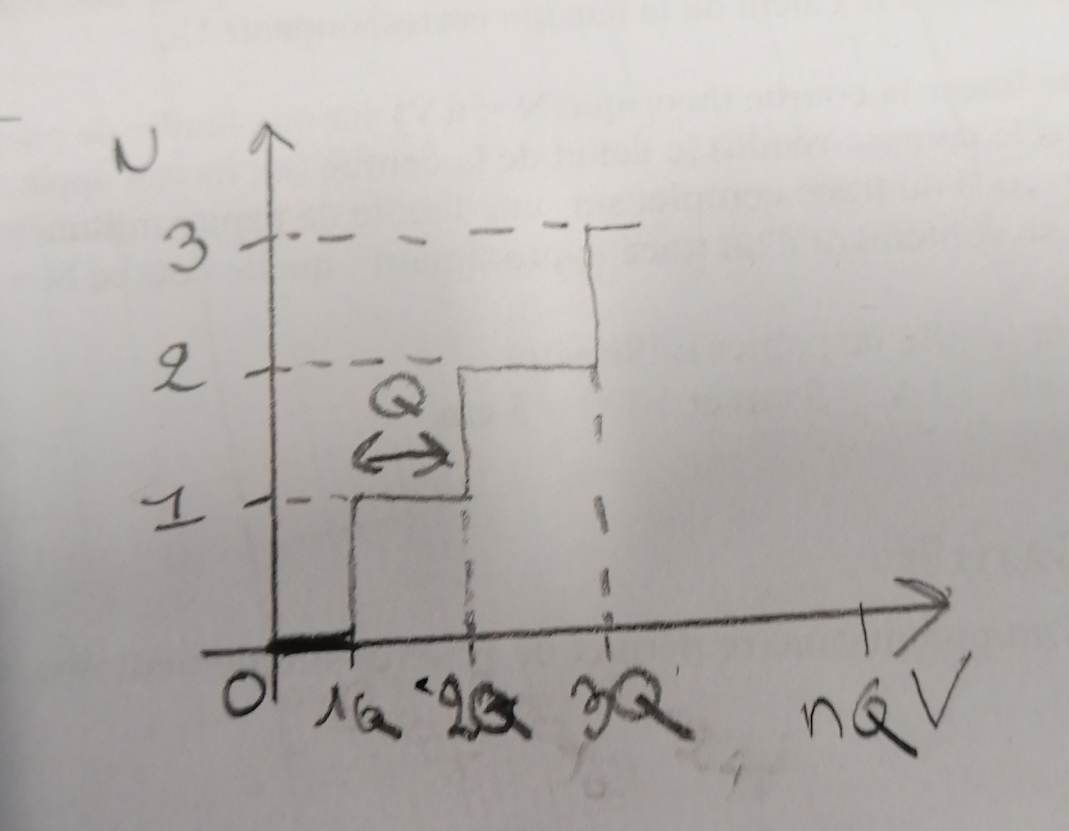
\includegraphics[scale=0.20]{image/1.jpg}
\caption{Courbe Rapide}
\label{fig:net }
\end{figure}


 Sur notre papier milimetré, nous ne pourrons tracer uniquement V/Q. En effet, tracer 4095 marches d'escalier sur la largeur d'une feuille A4 serait très long, très petit donc pas pertinant.
 
 
 \subsection{Courbe réelle}
 
 La resistance total du potentiometre est de 1k Ohms
 L'expression général de V est donc :\\
 
 V= ((xRT)/(xRT+(RT-xRT))).3,3V\\
 Simplication : x.3,3\\
 
 
 \begin{tabular}{|l|l|}
\hline
    V (mV) & N \\ \hline
    4,17 & 0   \\ \hline
    403 &  300 \\ \hline
    503 & 432 \\ \hline
    750 & 716 \\ \hline
    903 & 886 \\ \hline
    1 & 1016 \\ \hline
    1,20 & 1251\\ \hline
    1,30 & 1392 \\ \hline
    1,40 & 1516 \\ \hline
    1,50 & 1630 \\ \hline
    1,60 & 1762\\ \hline
    1,70&1901\\ \hline
    1,80&2000\\ \hline
    1,90& 2125\\ \hline
    2&2229\\ \hline
    2,10&2387\\ \hline
    2,20&2487\\ \hline
    2,30&2611\\ \hline
    2,40& 2714\\ \hline
    2,50& 2855\\ \hline
    2,60& 2979 \\ \hline
    2,70&3110\\ \hline
    2,80& 3250 \\ \hline
    2,90& 3431 \\ \hline
    3& 3615 \\ \hline
    3,10& 3815 \\ \hline
    3,20&4023\\ \hline
    3,30& 4095 \\ \hline

\hline
\end{tabular}

 \section{Analyse de la conversion}
Quand on trace la courbe theorique, et la courbe crée grace à nos relevés, on se rend compte que les valeurs attendus ne sont, à l'exection pour 0, et 3,3 V, pas respecté. De plus, on voit très bien que la courbe a un domaine de validité. En effet, mes resultats montrent que la courbe respecte une droite entre environ 1V et 2,5 V. A l'extremité de ces deux valeurs, on observe des erreurs de quantifications.  

\begin{figure}[h!]
\centering
\includegraphics[scale=0.10]{image/2.jpg}
\caption{Courbe Theorique et  Pratique }
\label{fig:net }
\end{figure}
\section{Correction}
Alors on prologe, la notre droite pour récupérer deux points. on Obtient b= -190 
Puis on prend un autre points pour caluler le coefficient directeur a:
\begin{equation}\label{xx}
\begin{split}
&f(3,4)=4000\\
&f(0)=-190\\
&a=\frac{f(3,4)-f(0)}{3,4-0}\\
&a=\frac{4190}{3,4}\\
&a=1232,35\\
&Donc\ N= 1232,35.V-190
\end{split}
\end{equation}
Puis on essaye de détérminer Nc
\begin{equation}\label{xx}
\begin{split}
&N-> V=\frac{N-b}{a}\\
&Nc=\frac{V}{Q}=\frac{1}{Q}.\frac{N-b}{a}\\
&Nc=1241.\frac{1232.V-190+190}{1232}\\
&Nc=1241.V
\end{split}
\end{equation}
\section{Calcul de la tension issuse de la conversion}
\begin{equation}\label{xx}
\begin{split}
 &Unc = QNc = \frac{3.3}{4096}.(1241.V)\\
 &Donc\ :\ Unc = \frac{3.3}{4096}.(1241.(\frac{N-b}{a})
\end{split}
\end{equation}
\section{Vérification}
Grâce à Unc, on peut donc verifié notre formule comme ceci :
\insertcode{code/Unc.ino}{code}
Nous ponvons donc vérifier que nous avons les bonnes valeurs affichés sur le port serieet sur notre Oscillo.


On peut supposer que les autres CAN ont le meme biais d'erreurs. On peut donc vérifier que les autres CAN Fonctionne correctement avec le meme algorithmes.
J'obtient d'ailleur sur le port A3 les mêmes résultats:
\begin{figure}[h!]
\centering
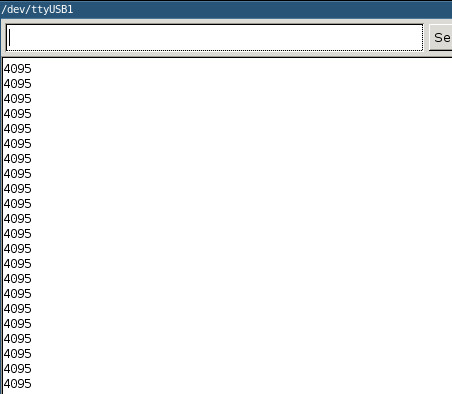
\includegraphics[scale=0.150]{image/3.jpg}
\caption{Courbe Rapide}
\label{fig:net }
\end{figure}\newpage


\section{Petit application Rapide}
\insertcode{code/angle.ino}{Ange}
\insertcode{code/serial.txt}{Sortie serie}


\section{applicationà une mesure de Température}
La dataSheet du TMP36:\url{http://cdn.sparkfun.com/datasheets/Sensors/Temp/TMP35_36_37.pdf}\\
Comment le brancher:\\ 
\begin{figure}[h!]
\centering
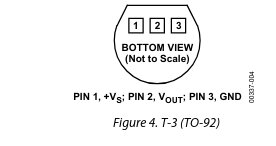
\includegraphics[scale=0.50]{image/4.jpg}
\caption{Comment brancher le TMP36}
\label{fig:net }
\end{figure}\\
La tension permise pour ce capteur est : [2.7V à 5.5V ]\\
Informations pèrtinantes:\\
\begin{figure}[h!]
\centering
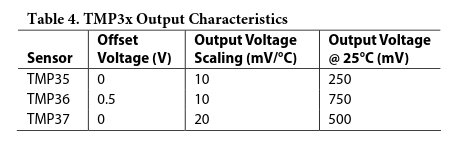
\includegraphics[scale=0.50]{image/5.jpg}
\caption{dataSheet}
\label{fig:net }
\end{figure}\\
\insertcode{code/tmp.ino}{Code pour le capteur de temperature}
Le moniteur serie:
\insertcode{code/serial.tmp}{temperature}
L'osiloscope et les valeurs ne sont pas coherent pour une raison toute simple, nous somme hors du domaine de validité du CAN, qui est compris entre 1V et 2,5V 
Grâce à la mesure direct via l'osciloscope nous donne une temperature de 26.4 C. 

Si l'on ne fais pas de correction voici les temperature que nous obtenons:
\insertcode{code/tmpUNUSE.ino}{On ne fais pas la correction du CAN} 
\insertcode{code/serialUNUSE.tmp}{Une temperature de 5 degres que fais l'IUT ?}



\end{document}

